
\documentclass[12pt]{article}

\usepackage[utf8]{inputenc}
\usepackage[T1]{fontenc}
\usepackage[polish,provide=*]{babel}
\usepackage{lmodern}
\usepackage{amsmath}
\usepackage{latexsym,amsfonts,amssymb,amsthm,amsmath}
\usepackage{enumitem}
\usepackage{hyperref}
\usepackage{graphicx}
\usepackage{float}
\usepackage{subcaption}
\usepackage{booktabs}
\graphicspath{{./images/}}

\setlength{\parindent}{0in}
\setlength{\oddsidemargin}{0in}
\setlength{\textwidth}{6.5in}
\setlength{\textheight}{8.8in}
\setlength{\topmargin}{0in}
\setlength{\headheight}{18pt}

\title{Wyznaczanie Współczynnika Załamania Światła w Pryzmacie}
\author{Kacper Kłos}

\begin{document}

\maketitle

W doświadczeniu zbadaliśmy zależność współczynnika załamania światła od długości fali oraz zaobserwowaliśmy zjawisko dwójłomności.
Wyznaczone współczynniki załamania dla kalcytu (materiału dwójłomnego) wykazują dużą zgodność z wartościami podawanymi w literaturze.
Stwierdziliśmy również, że zależność współczynnika załamania od długości fali można opisać za pomocą modeli Cauchy'ego oraz Sellmeiera.

\newpage

\section{Wstęp}
W niniejszym opracowaniu przedstawiamy metodę wyznaczania współczynnika załamania światła dla dwóch pryzmatów.  
W pierwszej części dokonujemy pomiaru współczynnika załamania szkła dla kilku wybranych długości fal (kolorów), co pozwala na obserwację dyspersji i dopasowanie wyników do powszechnie znanych modeli (Cauchego i Sellmeiera).  
W drugiej części analizujemy właściwości dwójłomne pryzmatu z kalcytu, wyznaczając współczynniki załamania dla promienia zwyczajnego oraz nadzwyczajnego przy wykorzystaniu odpowiedniej polaryzacji światła.
\section{Podstawy Teoretyczne}
\subsection{Kąt łamiący pryzmat}
Aby wyznaczyć kąt łamiący pryzmat, $\phi$, kierujemy wiązkę światła na jego wierzchołek i rozważamy odbite promienie. Zakładamy, że kąt padania jest równy kątowi odbicia (prawo odbicia).  
Konstrukcja geometryczna (rys.~\ref{fig:teoria_kat_lamiacy}) umożliwia nam wyznaczenie kąta łamiącego $\phi$ w oparciu o pomiar kąta $\psi$, pod którym rejestrujemy wiązkę odbitą dwukrotnie od ścian pryzmatu.  
Z zależności:
\[
    \phi = \phi_1 + \phi_2,\quad
    90^\circ = \alpha + \phi_{1},\quad 
    90^\circ = \beta + \phi_{2},\quad
    \psi = 2(\alpha + \beta),
\]
możemy otrzymać:
\[
    \phi = \frac{\psi}{2}.
\]

\begin{figure}[H]
    \centering
    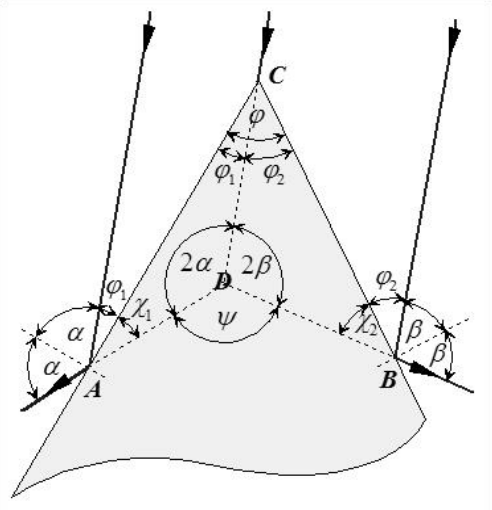
\includegraphics[scale=0.5]{teoria_kat_pryzmatu}
    \caption{Diagram ilustrujący wyznaczanie kąta łamiącego pryzmat $\phi$ (źródło: \cite{cwiczenie}).}
    \label{fig:teoria_kat_lamiacy}
\end{figure}

\subsection{Kąt najmniejszego odchylenia}
Analizując kąt odchylenia $\delta$, rozpatrujemy trajektorię promienia przechodzącego przez pryzmat (rys.~\ref{fig:teoria_kat_odchylenia}). Z prawa Snella oraz zależności geometrycznych wynika:  
\[
    \delta = \alpha_{1} + \alpha_{2} - \phi,
\]
przy czym
\[
    \alpha_{2} = \arcsin\bigl(n \sin(\phi - \arcsin(\tfrac{1}{n}\sin \alpha_1))\bigr).
\]
Do minimum kąta odchylenia $\delta_{\mathrm{min}}$ dochodzi, gdy $\alpha_{1} = \alpha_{2}$, co geometrycznie odpowiada sytuacji, w której promień wewnątrz pryzmatu biegnie symetrycznie. Finalnie otrzymujemy znany wzór na współczynnik załamania:
\begin{equation}
    n = \frac{\sin \alpha_{1}}{\sin \beta_{1}} 
    = \frac{\sin\bigl(\tfrac{1}{2}(\delta_{\mathrm{min}} + \phi)\bigr)}{\sin\bigl(\tfrac{1}{2}\phi\bigr)}.
    \label{eq:index}
\end{equation}
(Dokładne wyprowadzenie powyższego wzoru \cite{optics})

\begin{figure}[H]
    \centering
    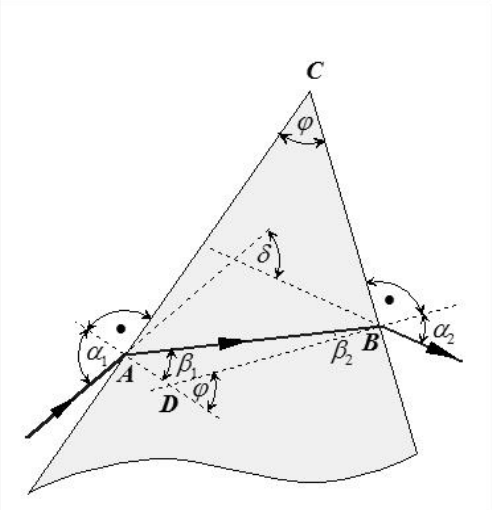
\includegraphics[scale=0.5]{teoria_kat_minimalny}
    \caption{Diagram dla wyznaczania kąta minimalnego odchylenia $\delta_{\mathrm{min}}$ (źródło: \cite{cwiczenie}).}
    \label{fig:teoria_kat_odchylenia}
\end{figure}

\subsection{Dyspersja i dwójłomność}
Podczas pomiarów zauważamy zjawisko dyspersji: światło rozszczepia się na poszczególne długości fal, z których każda charakteryzuje się nieco innym współczynnikiem załamania.  
W przypadku kryształów dwójłomnych (np. kalcytu) materiał wyróżnia dwa różne współczynniki załamania w zależności od polaryzacji światła – promień zwyczajny i nadzwyczajny rozchodzą się z różnymi prędkościami.

\section{Układ pomiarowy}
\subsection{Pomiar kąta łamiącego pryzmat}
W celu wyeliminowania błędów związanych z niedokładną kalibracją goniometru dokonujemy kilku pomiarów przy różnych orientacjach pryzmatu. Na rys.~\ref{fig:diagram_kat_pryzmatu} przedstawiamy widok z góry układu:  
\begin{itemize}[noitemsep]
    \item 1 – kolimator (z lampą helową),  
    \item 2 – pryzmat,  
    \item 3 – stół goniometru,  
    \item 4.1 i 4.2 – dwie pozycje lunety rejestrującej odbite promienie.
\end{itemize}
Z rozważań teoretycznych wiemy, że kąt $\phi$ możemy obliczyć ze wzoru:
\begin{equation}
    \phi = \begin{cases}
        \tfrac{1}{2}\,(\theta - \kappa), & \text{jeżeli } \theta > \kappa,\\
        \tfrac{1}{2}\,\bigl(360^\circ + \theta - \kappa\bigr), & \text{jeżeli } \theta < \kappa,
    \end{cases}
    \label{eq:lamiacy}
\end{equation}
gdzie $\theta$ i $\kappa$ to wskazania goniometru w dwóch położeniach lunety. Dodanie $360^\circ$ zapobiega otrzymaniu wartości ujemnej. Pomiar powtarzamy wielokrotnie, aby zmniejszyć ryzyko błędów.

\subsection{Pomiar kąta najmniejszego odchylenia}
W analogiczny sposób (rys.~\ref{fig:diagram_kat_minimalny}) dokonujemy pomiaru kąta najmniejszego odchylenia $\delta_{\mathrm{min}}$. Po chwili zastanowienia możemy zauważyć że wzór na $\delta_\mathrm{min}$ możemy przedstawić jako:
\begin{equation}
    \delta_\mathrm{min} = \begin{cases}
        \frac{1}{2}( \gamma - \zeta) \; \text{gdy }  \zeta > \gamma \\
        \frac{1}{2}(360^{\circ} - \gamma + \zeta) \; \text{gdy } \zeta < \gamma
    \end{cases}
    \label{eq:min}
\end{equation}
Również wykonujemy serię pomiarów, aby zredukować błędy systematyczne. 
Minimum kąta odchylenia rozpoznajemy po tym, że po niewielkim obracaniu stołu goniometru obraz rozszczepionego promienia w pewnym momencie przestaje się przesuwać, po czym zaczyna wracać w przeciwnym kierunku – ten punkt odpowiada $\delta_{\mathrm{min}}$.  
Jeżeli w pryzmacie dwójłomnym pojawiają się dwa rozdzielone widma, wtedy poprzez odpowiednie ustawienie polaryzatora ustawionego na kolimatorze, możemy „wybrać” jedną z polaryzacji (zwykłą lub nadzwyczajną).

\begin{figure}[H]
    \centering
    \begin{subfigure}{0.3\textwidth}
        \centering
        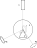
\includegraphics[width=\linewidth]{kat_pryzmatu}
        \caption{Diagram pomiaru kąta łamiącego.}
        \label{fig:diagram_kat_pryzmatu}
    \end{subfigure}
    \hspace{1in}
    \begin{subfigure}{0.3\textwidth}
        \centering
        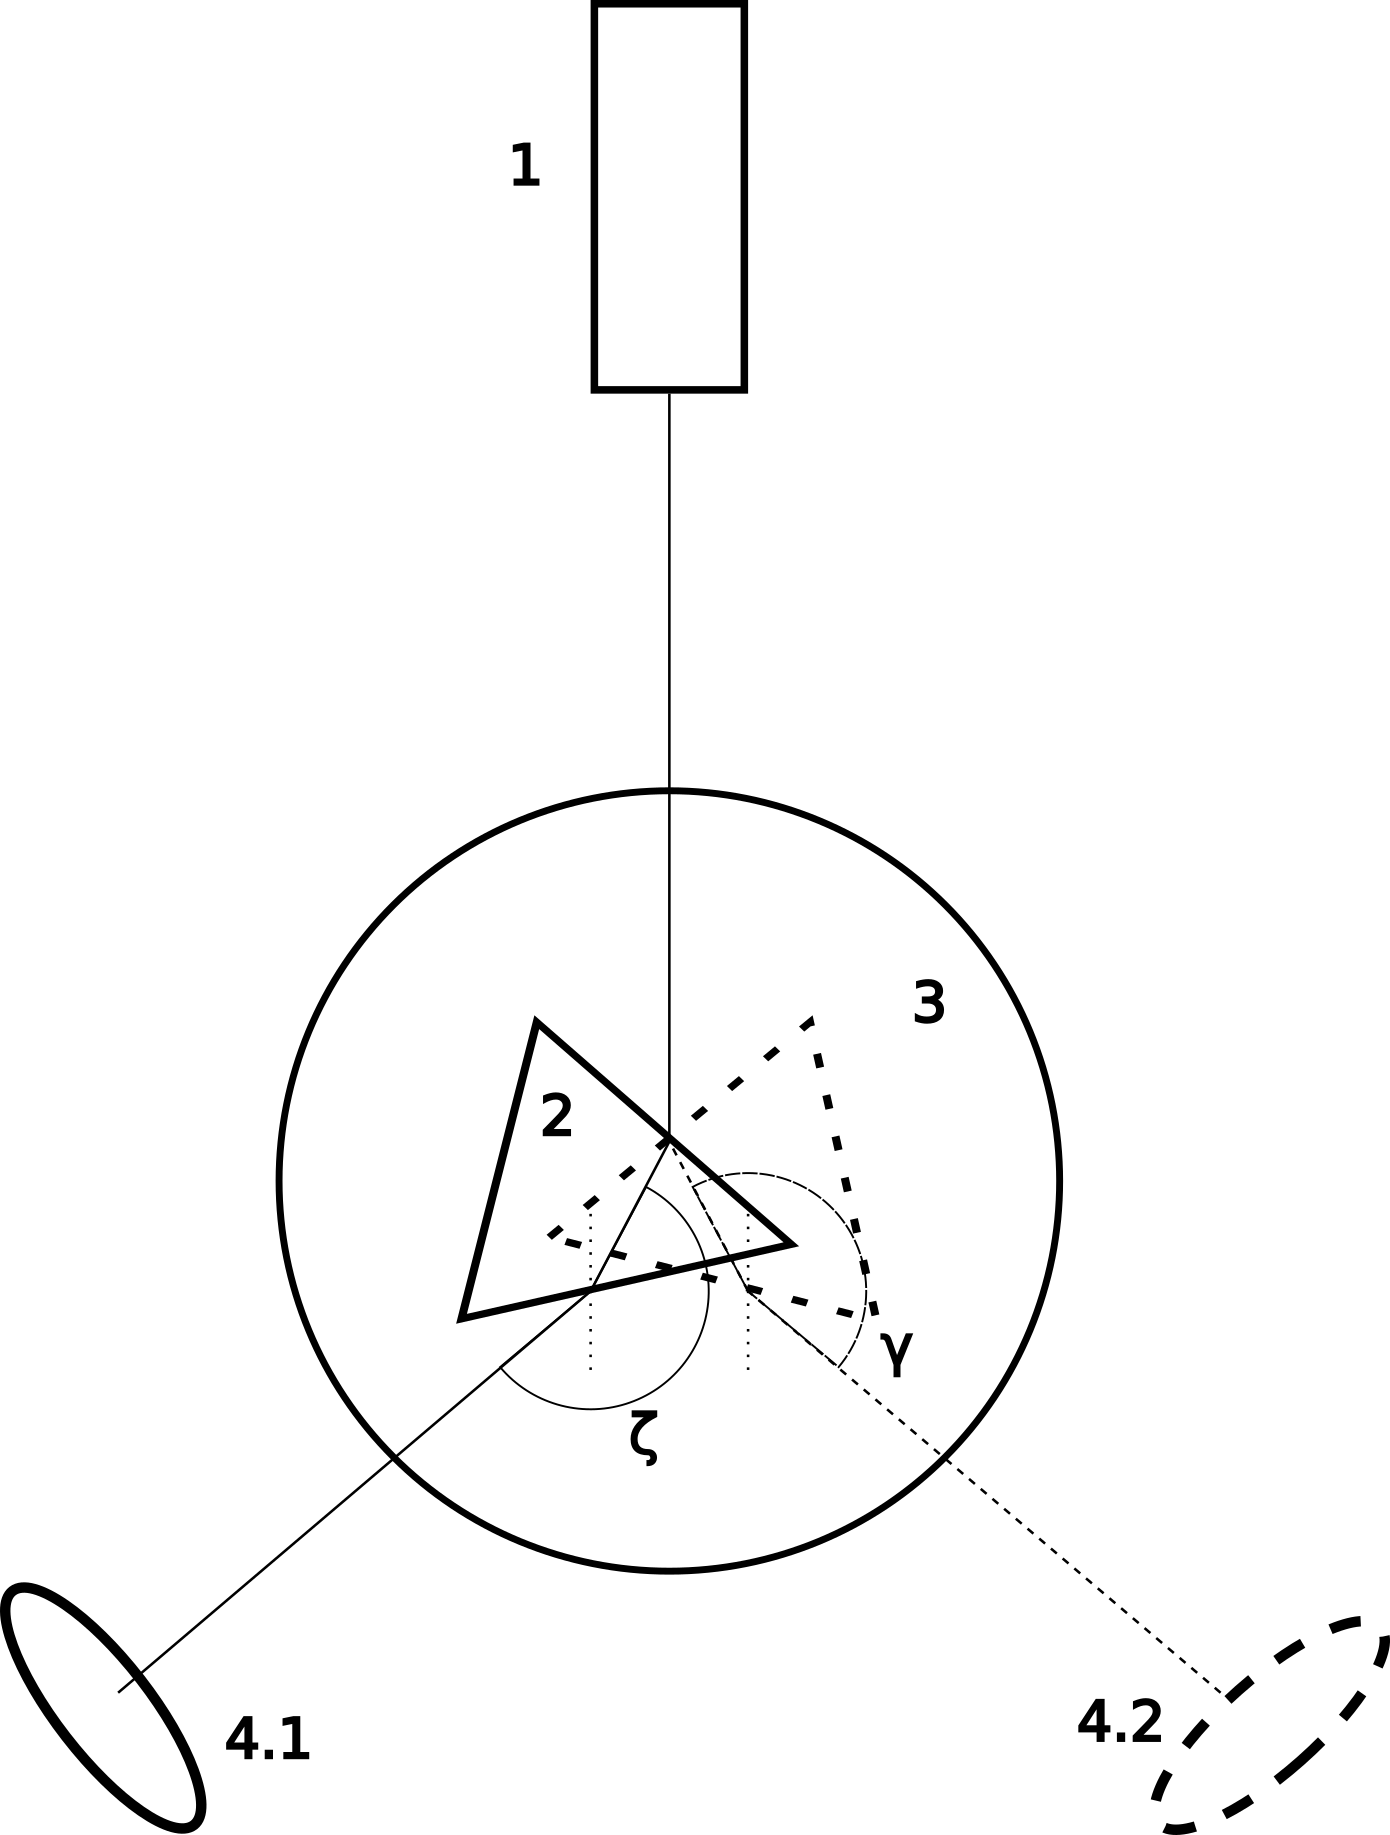
\includegraphics[width=\linewidth]{kat_minimalny}
        \caption{Diagram kąta najmniejszego odchylenia.}
        \label{fig:diagram_kat_minimalny}
    \end{subfigure}
    \caption{Diagramy układów doświadczalnych (rzut z góry)}
\end{figure}

\section{Wyniki pomiarów}

\subsection{Pryzmat szklany}

\begin{table}[H]
    \centering
    \begin{tabular}{c|ccc}
        \toprule
        \textbf{Nr} & $\theta_{s}$ & $\kappa_{s}$  & $\phi_{s}$ \\
        \midrule
        1 & 52°23'  & 322°22'  & 45°00'30'' \\
        2 & 40°38'  & 310°38'  & 45°00'00'' \\
        3 & 54°22'  & 324°20'  & 45°01'00'' \\
        4 & 38°18'  & 308°15'  & 45°01'30'' \\
        5 & 49°01'  & 319°59'  & 45°01'00'' \\
        6 & 58°23'  & 328°20'  & 45°01'30'' \\
        \bottomrule
    \end{tabular}
    \caption{Pomiary kątów odbitych przez pryzmat szklany.}
    \label{tab:katy_pryzmatu_szklo}
\end{table}

\begin{table}[H]
    \centering
    \begin{tabular}{c|ccc}
        \toprule
        \textbf{Nr} & $\zeta_{\mathrm{blue}}$ & $\gamma_{\mathrm{blue}}$  & $\delta_{\mathrm{blue}}$ \\
        \midrule
        1 & 35°30'  & 321°29'  & 37°00'30'' \\
        2 & 35°30'  & 321°27'  & 37°01'30'' \\
        3 & 35°30'  & 321°29'  & 37°00'30'' \\
        4 & 35°30'  & 321°28'  & 37°01'00'' \\
        \bottomrule
    \end{tabular}
    \caption{Pomiar najmniejszego kąta odchylenia dla koloru niebieskiego (pryzmat szklany).}
    \label{tab:katy_odchylenia_szkło_niebieski}
\end{table}

\begin{table}[H]
    \centering
    \begin{tabular}{c|ccc}
        \toprule
        \textbf{Nr} & $\zeta_{\mathrm{green}}$ & $\gamma_{\mathrm{green}}$  & $\delta_{\mathrm{green}}$ \\
        \midrule
        1 & 34°45'  & 322°15'  & 36°15'00'' \\
        2 & 34°45'  & 322°14'  & 36°15'30'' \\
        3 & 34°45'  & 322°13'  & 36°16'00'' \\
        4 & 34°45'  & 322°13'  & 36°16'00'' \\
        \bottomrule
    \end{tabular}
    \caption{Pomiar najmniejszego kąta odchylenia dla koloru zielonego (pryzmat szklany).}
    \label{tab:katy_odchylenia_szkło_zielony}
\end{table}

\begin{table}[H]
    \centering
    \begin{tabular}{c|ccc}
        \toprule
        \textbf{Nr} & $\zeta_{\mathrm{yellow}}$ & $\gamma_{\mathrm{yellow}}$  & $\delta_{\mathrm{yellow}}$ \\
        \midrule
        1 & 34°02'  & 322°56'  & 35°33'00'' \\
        2 & 34°02'  & 322°56'  & 35°33'00'' \\
        3 & 34°02'  & 322°56'  & 35°33'00'' \\
        4 & 34°01'  & 322°57'  & 35°32'00'' \\
        \bottomrule
    \end{tabular}
    \caption{Pomiar najmniejszego kąta odchylenia dla koloru żółtego (pryzmat szklany).}
    \label{tab:katy_odchylenia_szkło_zolty}
\end{table}

\begin{table}[H]
    \centering
    \begin{tabular}{c|ccc}
        \toprule
        \textbf{Nr} & $\zeta_{\mathrm{red}}$ & $\gamma_{\mathrm{red}}$  & $\delta_{\mathrm{red}}$ \\
        \midrule
        1 & 33°36'  & 323°21'  & 35°07'30'' \\
        2 & 33°36'  & 323°21'  & 35°07'30'' \\
        3 & 33°36'  & 323°22'  & 35°07'00'' \\
        4 & 33°37'  & 323°21'  & 35°08'00'' \\
        \bottomrule
    \end{tabular}
    \caption{Pomiar najmniejszego kąta odchylenia dla koloru czerwonego (pryzmat szklany).}
    \label{tab:katy_odchylenia_szkło_czerwony}
\end{table}

\subsection{Pryzmat kalcytowy}

\begin{table}[H]
    \centering
    \begin{tabular}{c|ccc}
        \toprule
        \textbf{Nr} & $\theta_{k}$ & $\kappa_{k}$  & $\phi_{k}$ \\
        \midrule
        1 & 65°38'  & 305°22'  & 60°08'00'' \\
        2 & 79°20'  & 319°03'  & 60°08'30'' \\
        3 & 89°29'  & 329°11'  & 60°09'00'' \\
        4 & 56°09'  & 295°55'  & 60°07'30'' \\
        \bottomrule
    \end{tabular}
    \caption{Pomiary kątów odbitych przez pryzmat z kalcytu.}
    \label{tab:katy_pryzmatu_kalcyt}
\end{table}

\begin{table}[H]
    \centering
    \begin{tabular}{c|ccc|ccc}
        \toprule
        \textbf{Nr} & $\zeta_{\mathrm{zwy}}$ & $\gamma_{\mathrm{zwy}}$ & $\delta_{\mathrm{zwy}}$ & $\zeta_{\mathrm{nadzwy}}$ & $\gamma_{\mathrm{nadzwy}}$ & $\delta_{\mathrm{nadzwy}}$ \\
        \midrule
        1 & 34°31'  & 322°19'  & 36°06'00'' & 50°42'  & 306°14'  & 52°14'00'' \\
        2 & 34°31'  & 322°18'  & 36°06'30'' & 50°42'  & 306°15'  & 52°13'30'' \\
        3 & 34°31'  & 322°18'  & 36°06'30'' & 50°42'  & 306°14'  & 52°14'00'' \\
        \bottomrule
    \end{tabular}
    \caption{Pomiar najmniejszego odchylenia dla pryzmatu z kalcytu (linia żółta helu) – wartości dla promienia zwyczajnego i nadzwyczajnego.}
    \label{tab:katy_odchylenia_kalcyt}
\end{table}

\section{Wyniki i analiza błędu}
Dla każdego pomiaru wyznaczamy wartości średnie oraz niepewności (błąd statystyczny i tzw. błąd całkowity), zakładając dla goniometru niepewność odczytu równą połowie podziałki, zatem $30''$.  
W poniźszej analizie $s_x$ oznacza błąd statystyczny pomiaru wartości $x$, $\Delta(x)$ to błąd pomiarowy $x$, a $u(x)$ symbolizuje sumaryczny błąd dla $x$.
Wzór na propagację błędu dla funkcji $f(x_1,\ldots,x_i)$ wyrażamy standardową zależnością:

\begin{equation}
    \Delta f = \sqrt{\left(\frac{\partial f}{\partial x_1}\Delta x_1\right)^2 + \dots + \left(\frac{\partial f}{\partial x_i}\Delta x_i\right)^2}.
    \label{eq:error_propagation}
\end{equation}

A cała niepewność będzie miała dla nas konserwatywną postać:

\begin{equation}
    u(x) = \sqrt{s^2_x + \Delta(x)^2}
    \label{eq:full_error}
\end{equation}

Gdzie dla wzoru \eqref{eq:index} pochodne mają postać:

\begin{equation}
    \frac{\partial n}{\partial \delta_{\mathrm{min}}} = \frac{\cos(\frac{1}{2}(\delta_{\mathrm{min}}+\phi))}{2\sin(\frac{\phi}{2})}, \quad
    \frac{\partial n}{\partial \phi} = -\frac{\sin(\frac{\delta_{\mathrm{min}}}{2})}{2\sin^2(\frac{\phi}{2})}
    \label{eq:index_err}
\end{equation}

Dla kąta łamiącego i kąta najmniejszego odchylenia opisanych wedle wzorów \eqref{eq:lamiacy}\eqref{eq:min} otrzymujemy błędy: 

\[
    \Delta(\phi) = \frac{\Delta}{\sqrt{2}}, \quad
    \Delta(\delta_{\mathrm{min}}) = \frac{\Delta}{\sqrt{2}}.
\]
($\Delta$ we wzorze jest błędem pomiarowym goniometru.)

W przypadku pryzmatu szklanego używając danych z (tab.~\ref{tab:katy_pryzmatu_szklo}) wraz ze wzorem \eqref{eq:full_error}, otrzymaliśmy wartości średnie:

\[
    \bar{\phi}_{s} \approx 45^\circ00'55'' \quad (s_{\phi_{s}} = 14'',\; u(\phi_{s}) = 26''),
\]

zaś dla pryzmatu z kalcytu dla zanych (tab.~\ref{tab:katy_pryzmatu_kalcyt}) ponownie korzystająz ze wzoru \eqref{eq:full_error}, mamy:

\[
    \bar{\phi}_{k} \approx 60^\circ08'15'' \quad (s_{\phi_{k}} = 19'',\; u(\phi_{k}) = 28'').
\]

Mając do dyspozycji $\phi$ i zmierzone wartości $\delta_{\mathrm{min}}$ w (tab.~\ref{tab:katy_odchylenia_szkło_niebieski},~\ref{tab:katy_odchylenia_szkło_zielony},~\ref{tab:katy_odchylenia_szkło_zolty},~\ref{tab:katy_odchylenia_szkło_czerwony}), (tab.~\ref{tab:katy_odchylenia_kalcyt})
oraz wszystkie wzory \eqref{eq:index}\eqref{eq:error_propagation}\eqref{eq:full_error}\eqref{eq:index_err} wyznaczamy ostatecznie współczynniki załamania wraz z ich niepewnościami:

\begin{table}[H]
    \centering
    \begin{tabular}{c|ccccc}
        \toprule
        \textbf{Kolor} & $\delta_{\mathrm{min}}$ & $s_{\delta}$ & $u(\delta_{\mathrm{min}})$ & $n_{s}$ & $u(n_{s})$ \\
        \midrule
        Niebieski & 37°00'53'' & 14'' & 26'' & 1{,}71433 & 0{,}00018 \\
        Zielony   & 36°15'38'' & 14'' & 26'' & 1{,}70132 & 0{,}00018 \\
        Żółty     & 35°32'45'' & 15'' & 26'' & 1{,}68892 & 0{,}00018 \\
        Czerwony  & 35°07'30'' & 12'' & 25'' & 1{,}68159 & 0{,}00018 \\
        \bottomrule
    \end{tabular}
    \caption{Wyniki dla pryzmatu szklanego: najmniejszy kąt odchylenia, współczynnik załamania i niepewność.}
    \label{tab:szklo_tabela}
\end{table}

\begin{table}[H]
    \centering
    \begin{tabular}{c|ccccc}
        \toprule
        & $\delta_{\mathrm{min}}$ & $s_{\delta}$ & $u(\delta_{\mathrm{min}})$ & $n_{\mathrm{zwy}}$ / $n_{\mathrm{nadzwy}}$ & $u(n)$ \\
        \midrule
        Promień zwyczajny    & 36°06'20'' & 10'' & 23'' & 1{,}48604 & 0{,}00012 \\
        Promień nadzwyczajny & 52°13'50'' & 10'' & 23'' & 1{,}65821 & 0{,}00014 \\
        \bottomrule
    \end{tabular}
    \caption{Wyniki dla pryzmatu z kalcytu (linia żółta, $\lambda \approx 587{,}5\,\mathrm{nm}$).}
    \label{tab:kalcyt_tabela}
\end{table}

\noindent
Dla pryzmatu kalcytowego otrzymane wartości (tab.~\ref{tab:kalcyt_tabela}) porównaliśmy z wynikami znanymi z literatury \cite{kalcyt} (Bragg i Gibbs): 

\[
    n_{\mathrm{zwy}} \approx 1{,}486, \quad n_{\mathrm{nadzwy}} \approx 1{,}658, 
\]

co wykazuje dobrą zgodność w granicach niepewności.

\subsection{Identyfikacja długości fal i dopasowanie modeli}

Mierząc linie widmowe helu \cite{linie_1,linie_2} oraz obserwując intensywność, zidentyfikowaliśmy mierzone długości fal na: 

\[
    \lambda_{\mathrm{blue}} = 447{,}1\,\mathrm{nm}, \quad
    \lambda_{\mathrm{green}} = 501{,}5\,\mathrm{nm}, \quad
    \lambda_{\mathrm{yellow}} = 587{,}5\,\mathrm{nm}, \quad
    \lambda_{\mathrm{red}} = 667{,}8\,\mathrm{nm}.
\]

Na rys.~\ref{fig:linie_helu} przedstawiamy przykładowy schemat linii widmowych helu \cite{obraz_linie}.

\begin{figure}[H]
    \centering
    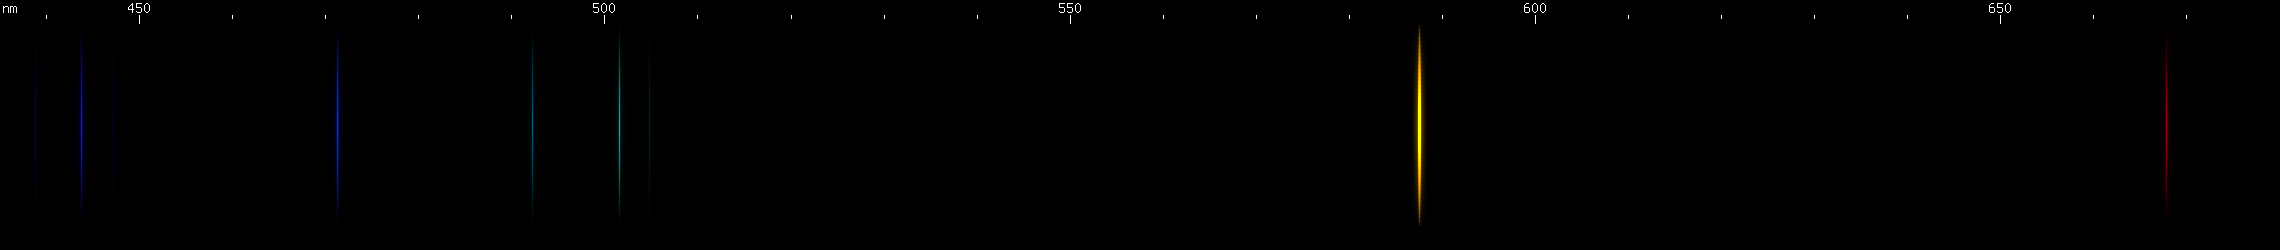
\includegraphics[width=0.90\textwidth]{He I}
    \caption{Przykładowe linie widmowe helu; w pomiarze zarejestrowaliśmy najjaśniejsze spośród nich (źródło: \cite{obraz_linie}).}
    \label{fig:linie_helu}
\end{figure}

Dane z tabeli \ref{tab:szklo_tabela} wskazują na wyraźną dyspersję współczynnika załamania w zakresie $\lambda \in [447{,}1\,\mathrm{nm},\,667{,}8\,\mathrm{nm}]$, mieszczącą się w przedziale $n \in [1{,}68159;\,1{,}71433] \pm 0{,}00018$.  
Prowadzi to nas do wniosku że materiał z którego został wykonany pryzmat szklany to najprawdopodobniej pewien rodzaj szkła N-SF5 mające nieznacznie mniejszy współczynnik załamania \cite{szklo} dla badanego przez nas spektrum.

Przeprowadziliśmy dopasowanie do dwóch popularnych modeli:  
\[
    n_{\mathrm{Cauchy}}(\lambda) = A_0 + \frac{A_1}{\lambda^2}, 
\]
\[
    n_{\mathrm{Sellmeier}}^2(\lambda) = 1 + \frac{B_1\,\lambda^2}{\lambda^2 - C_1}.
\]
Po zastosowaniu metody najmniejszych kwadratów otrzymaliśmy wartości:
\[
    A_0 = 1{,}6547,\quad u(A_0) = 9\times 10^{-4}, \qquad A_1 = 1{,}18\times 10^{-14}\,\mathrm{m^2}, \quad u(A_1) = 3 \times 10^{-16}\,\mathrm{m^2}
\]
\[
    B_1 = 1{,}7461,\quad u(B_1) = 1{,}4\times 10^{-3},\qquad C_1 = 1{,}98\times 10^{-8}\,\mathrm{m^2},\quad u(C_1) = 2\times 10^{-10}\,\mathrm{m^2},
\]
Wraz z macierzami kowariantnymi:
\[
    K_{Cauchy} = \begin{bmatrix}
        7{,}3 \cdot 10^{-6} & -1{,}9 \cdot 10^{-19} \, \mathrm{m^2} \\
        -1{,}9 \cdot 10^{-19} \, \mathrm{m^2} & 5{,}4 \cdot 10^{-32} \, \mathrm{m^4}
    \end{bmatrix}
\]
\[
    K_{Sellmeier} = \begin{bmatrix}
        1{,}8 \cdot 10^{-6} & -2{,}4 \cdot 10^{-13} \, \mathrm{m^2} \\
        -2{,}4 \cdot 10^{-13} \, \mathrm{m^2} & 3{,}6 \cdot 10^{-20} \, \mathrm{m^4}
    \end{bmatrix}
\]
Punkty pomiarowe wraz z dopasowanymi krzywymi zwizualizowaliśmy na (rys.~\ref{fig:wykres}).

\begin{figure}[H]
    \centering
    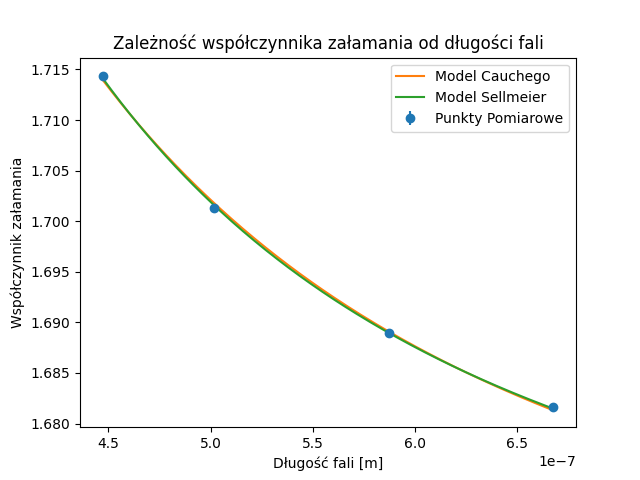
\includegraphics[scale=0.9]{wykres}
    \caption{Wyznaczone doświadczalnie punkty pomiarowe (z naniesionymi błędami) oraz dopasowane krzywe modeli Cauchego i Sellmeiera.}
    \label{fig:wykres}
\end{figure}

Należy jednak pamiętać, że wyznaczone punkty pomiarowe nie są całkowicie niezależne.
Wartość każdego punktu jest wyznaczana na podstawie wcześniej obliczonego kąta łamiącego pryzmatu, co wprowadza pewien rodzaj błędu systematycznego do naszych pomiarów.
Mimo to dopasowanie punktów do wspomnianych modeli wciąż daje nam cenne informacje na temat ich skuteczności.

Test $\chi^2$ pozwala stwierdzić, że w tym przypadku lepsze dopasowanie zapewnia model Sellmeiera:
\[
    \chi^{2}_{\text{Cauchy}} = 14{,}74
\]
\[
    \chi^{2}_{\text{Sellmeier}} = 4{,}13
\]

Analizując wyniki testu $\chi^2$ dla liczby stopni swobody $dof=2$, zauważamy, że żaden z modeli nie jest w stanie precyzyjnie przewidzieć zmierzonych wartości. 
Należy jednak uwzględnić wspomniany wcześniej błąd systematyczny wynikający z wyznaczenia kąta łamiącego, który może znacząco wpływać na uzyskane przez nas dopasowanie.


\newpage

\section{Podsumowanie}
W przeprowadzonych badaniach wyznaczyliśmy współczynniki załamania światła w pryzmacie szklanym dla kilku długości fal (kolorów światła z lampy helowej) oraz w pryzmacie kalcytowym (rozróżniając promień zwyczajny i nadzwyczajny).  
W przypadku szkła współczynnik załamania w zakresie $\lambda \in [447{,}1\,\mathrm{nm},\,667{,}8\,\mathrm{nm}]$ mieści się w przedziale $n \in [1{,}68159;\,1{,}71433] \pm 0{,}00018$, co świadczy o silnej dyspersji materiału.
Dopasowanie do modeli Cauchego i Sellmeiera pokazało, że w badanym zakresie długości fal model Sellmeiera lepiej opisuje zależność $n(\lambda)$.  
Dla kalcytu uzyskaliśmy wartości $n_{\mathrm{zwy}} = 1{,}48604 \pm 0{,}00012$ i $n_{\mathrm{nadzwy}} = 1{,}65821 \pm 0{,}00014$, co jest w bardzo dobrej zgodności z danymi literaturowymi \cite{kalcyt}.  
Wyniki potwierdzają zarówno zjawisko dyspersji, jak i dwójłomności. Zaprezentowana metoda pomiaru z użyciem goniometru i lampy helowej pozwala osiągnąć wysoką dokładność pomiarową oraz zweryfikować modele teoretyczne opisujące załamanie światła.

\newpage
\begin{thebibliography}{6}

\bibitem{cwiczenie}
\emph{Wyznaczanie Współczynników Załamania Światła w Pryzmacie}, Wydział Fizyki Uniwersytetu Warszawskiego.

\bibitem{optics}
Eugene Hecht, \emph{Optics}.

\bibitem{kalcyt}
W. L. Bragg, \emph{The Refractive Indices of Calcite and Aragonite}.

\bibitem{linie_1}
N. Abramzon, P. B. Siegel, \emph{Introductory Helium Atomic Spectrum Analysis}.

\bibitem{linie_2}
\url{https://physics.nist.gov/PhysRefData/Handbook/Tables/heliumtable2.htm}

\bibitem{obraz_linie}
\url{https://www.atomic-spectra.net}

\bibitem{szklo}
\url{https://refractiveindex.info/?shelf=specs&book=SCHOTT-optical&page=SF5}

\end{thebibliography}

\end{document}

